%%!TeX program = xelatex
%% 부득이하게 pdflatex을 사용해야 할 경우 위의 magic comment를 제거하십시오.

% Initiated by 정민석(2014년도 경기과학고 수학과전문교원)
% Continously being modified by 경기과학고 TeX 사용자협회
% Website : http://gshslatexintro.github.io 

\documentclass{new_report}
% 아래의 함수를 사용하면 이미지 파일들을 같은 디렉토리 내에 images 라는 이름을 가진 폴더를 생성한 후, 그 폴더 안에 넣어 사용할 수 있습니다.
% 사용하고자 한다면 주석을 푸십시오.
\graphicspath{{images/}}
% 이곳에 필요한 별도의 패키지들을 적어넣으시오.
%\usepackage{...}
\usepackage{verbatim} % for commment, verbatim environment
\usepackage{spverbatim} % automatic linebreak verbatim environment
%\usepacakge{indentfirst}
\usepackage{tikz}
%\tikzset{
%	image label/.style={
%		every node/.style={
			%fill=black,
			%text=white,
%			font=\sffamily\scriptsize,
%			anchor=south west,
%			xshift=0,
%			yshift=0,
%			at={(0,0)}
%		}
%	}
%}
\usepackage{amsmath}
\usepackage{amsfonts}
\usepackage{amssymb}
\usepackage{float}
\usepackage{graphicx}
\usepackage{tabularx}
\usepackage{multirow}
\usepackage{booktabs}
\usepackage{longtable}
\usepackage{gensymb}
\usepackage{wrapfig}
\usepackage{subcaption}
%\usepackage{floatrow}
%\usepackage{pict2e}
%\usepackage[backend=biber,style=authoryear]{biblatex}
%\usepackage{biblatex}
\usepackage{pgfplots}
\pgfplotsset{
	compat=newest,
	label style={font=\sffamily\scriptsize},
	ticklabel style={font=\sffamily\scriptsize},
	legend style={font=\sffamily\tiny},
	major tick length=0.1cm,
	minor tick length=0.05cm,
	every x tick/.style={black},
}

\usetikzlibrary{shapes}
\usetikzlibrary{plotmarks}
\usepackage{listings}
\usepackage{hologo}
\usepackage{makecell}

\lstset{
	basicstyle=\small\ttfamily,
	columns=flexible,
	breaklines=true
}

\citation
\bibdata

%: ----------------------------------------------------------------------
%:               보고서 정보를 입력하시오
% ----------------------------------------------------------------------
% 아래와 같은 command를 만들면 길이가 긴 용어를 간편하게 사용할 수 있습니다. 단, 이미 지정된 함수명들은 새로운 함수명으로 사용할 수 없습니다.
\newcommand{\gshs}{Gyeonggi Science High School for the Gifted }

\researchtype{} % 기초 / 심화
\reporttype{} % 중간 / 결과

\title{천체망원경 모터 포커서 컨트롤러 구동 시스템 및 ASCOM 드라이버 개발 } % 제목 개행 시 \linebreak 사용. \\나 \newline 은 안됨.
\englishtitle{English title}% 제목 개행 시 \linebreak 사용. \\나 \newline 은 안됨.

\author[1] {} % 제 1 저자명
\email[1]{} % 제 1 저자 이메일
\author[2] {} % 제 2 저자명
\email[2]{} % 제 2 저자 이메일
\advisor{} % 지도교사명
\advisorEmail{} % 지도교사 이메일

%%%%%%%%%%%%%%%%%%%%%%%%%%%%%%%%%%%%%%%%%%%%%%%
%%%% researchtype이 '심화'일 경우에만 나타남 %%%%
\professor{} % 지도교수명
\professorEmail{} % 지도교수 이메일
%%%%%%%%%%%%%%%%%%%%%%%%%%%%%%%%%%%%%%%%%%%%%%%%
\summitdate{}{}{} % 제출일 (연, 월, 일)
\newtheorem{definition}{정의}
 % usepackage 등의 명령어는 여기에.
\usepackage{cite}
\usepackage{textcomp}
\usepackage{tocloft}
\setlength{\cftbeforesecskip}{0pt}
\setlength{\cftbeforesubsecskip}{0pt}
\setlength{\cftbeforesubsubsecskip}{0pt}

% 본문 시작
\begin{document}

	%표지만들기
	%makecover 함수와 관련하여 "Underfull \hbox (badness 10000) in paragraph" 오류는 무시하십시오. (TeXstudio ver 2.9.4 오류 기준)
	%\makecover
	
	%\baselineskip=2.2em         % line spacing in the paragraph
	\maketitle  % command to print the title page with above variables
\setcounter{page}{1}
%---------------------------------------------------------------------
%                  영문 초록을 입력하시오
%---------------------------------------------------------------------
\begin{abstracts}     %this creates the heading for the abstract page
	\addcontentsline{toc}{section}{Abstract}  %%% TOC에 표시
	\noindent{
	초록(요약문)은 가장 마지막에 작성한다. 연구한 내용, 즉 본론부터 요약한다. 서론 요약은 하지 않는다. 대개 첫 문장은 연구 주제 (+방법을 핵심적으로 나타낼 수 있는 문구: 실험적으로, 이론적으로, 시뮬레이션을 통해)를 쓴다. 다음으로 연구 방법을 요약한다. 선행 연구들과 구별되는 특징을 중심으로 쓴다. 뚜렷한 특징이 없다면 연구방법은 안써도 상관없다. 다음으로 연구 결과를 쓴다. 연구 결과는 추론을 담지 않고, 객관적으로 서술한다. 마지막으로 결론을 쓴다. 이 연구를 통해 주장하고자 하는 바를 간략히 쓴다. 요약문 전체에서 연구 결과와 결론이 차지하는 비율이 절반이 넘도록 한다. 읽는 이가 요약문으로부터 얻으려는 정보는 연구 결과와 결론이기 때문이다. 연구 결과만 레포트하는 논문인 경우, 결론을 쓰지 않는 경우도 있다.
		
		key word : Telescope
	}
\end{abstracts}

\begin{abstractskor}
	본 연구는 소형 천체망원경의 아크릴 바흐티노프마스크 원격제어가 가능한 제어시스템인 GS-system를 개발하였다. GS-system은 기존에 개발한 모터포커서를 사용하되, 바흐티노프마스크의 원격 제어 및 다른 여러 기능을 탑재하여 사용의 편의성을 증대시켰으며, 이를 사용하여 특정 소형 천체망원경에 사용할 수 있는 바흐티노프마스크 제어용 덮개를 제어할 수 있도록 하였다. GS-system을 통해 소형 천체망원경에 사용되는 바흐티노프마스크의 제어를 편리하게 할 수 있으며, 천체 관측에 필요한 기능들 또한 ASCOM 드라이버와 호환되는 소프트웨어들을 통한 GUI (graphical user interface)를 활용해 편리하게 사용할 수 있도록 하였다. 
	
	키워드 : 자동망원경
	
\end{abstractskor}
%----------------------------------------------
%   Table of Contents (자동 작성됨)
%----------------------------------------------
\cleardoublepage
\addcontentsline{toc}{section}{Contents}
\setcounter{secnumdepth}{3} % organisational level that receives a numbers
\setcounter{tocdepth}{3}    % print table of contents for level 3
\baselineskip=2.2em
\tableofcontents


%----------------------------------------------
%     List of Figures/Tables (자동 작성됨)
%----------------------------------------------
\cleardoublepage
\clearpage
\listoffigures	% 그림 목록과 캡션을 출력한다. 만약 논문에 그림이 없다면 이 줄의 맨 앞에 %기호를 넣어서 코멘트 처리한다.

\cleardoublepage
\clearpage
\listoftables  % 표 목록과 캡션을 출력한다. 만약 논문에 표가 없다면 이 줄의 맨 앞에 %기호를 넣어서 코멘트 처리한다.

%%%%%%%%%%%%%%%%%%%%%%%%%%%%%%%%%%%%%%%%%%%%%%%%%%%%%%%%%%%
%%%% Main Document %%%%%%%%%%%%%%%%%%%%%%%%%%%%%%%%%%%%%%%%
%%%%%%%%%%%%%%%%%%%%%%%%%%%%%%%%%%%%%%%%%%%%%%%%%%%%%%%%%%%
\cleardoublepage
\clearpage
\renewcommand{\thepage}{\arabic{page}}
\setcounter{page}{1}



 % Abstract
	
	%%%%%%%%%%%%%%%%%%%%%%%%%%%%%%%%%%%%%%%%%%%%%%%%%%%%%%%%%%%
	%%%% Main Document %%%%%%%%%%%%%%%%%%%%%%%%%%%%%%%%%%%%%%%%
	%%%%%%%%%%%%%%%%%%%%%%%%%%%%%%%%%%%%%%%%%%%%%%%%%%%%%%%%%%%
	\cleardoublepage
	\clearpage
	\renewcommand{\thepage}{\arabic{page}}
	\setcounter{page}{1}
	
	%각 장을 아래와 같이 sub 폴더 안에 만들어서 넣으면 편리하다.
	\section{서론}

\subsection{연구의 필요성}

최근에는 천체 망원경이 대중화 되어 관측을 즐기는 인구가 많아 졌으며, 개인이 천체 망원경을 소유하여 장시간 노출을 필요로 하는 천체 사진 촬영을 즐기는 아마추어 천문인들도 온라인과 오프라인 동호회를 중심으로 많아지고 있다. Figure \ref{fig:The_Andromeda_Galaxy}\은 아마추어 천문가가 소형 천체망원경을 촬영한 안드로메다 은하의 사진이다. 이런 천체 사진을 촬영하기 위해서는 많은 노력이 필요하다.
\begin{figure}[h]
	\begin{center}
		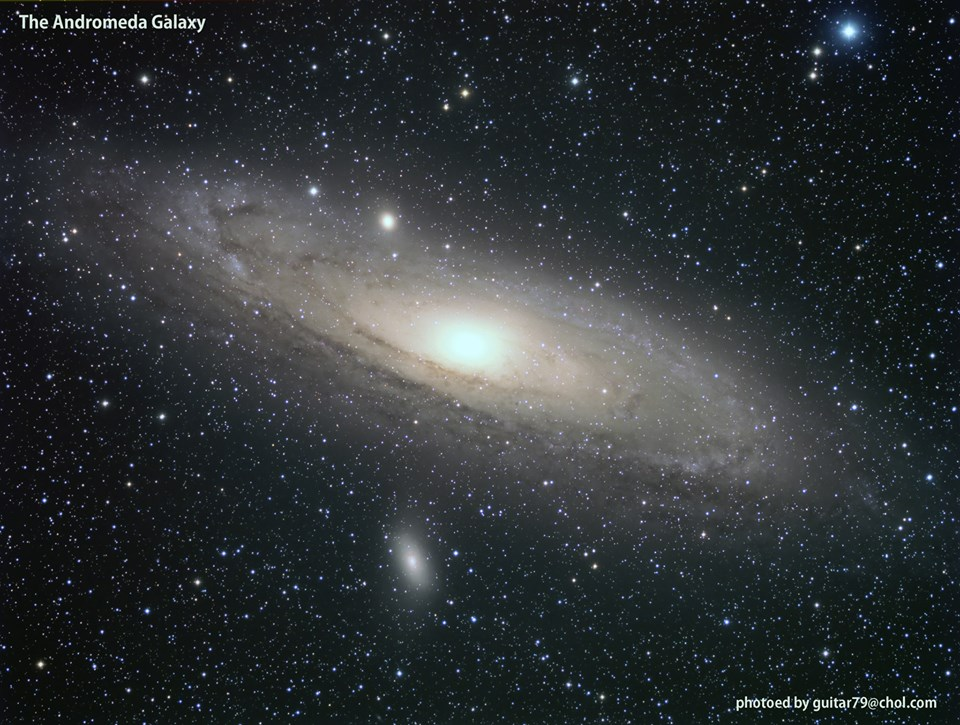
\includegraphics[width=0.95\linewidth]{Andromeda_Galaxy}
		\caption{The Andromeda Galaxy (Takahashi FSQ106-ED with 0.73X Reducer QE, Sbig ST-8300M, Takahashi EM-200 Temma 2) : L 600s X 14 frames, RGB 400s X 6 frames each.}
		\label{fig:The_Andromeda_Galaxy}
	\end{center}
\end{figure}

Figure \ref{fig:observing_system}\은 사진 관측을 하기 위한 천체 망원경 시스템을 보여 준다. 사진 관측을 위한 천체 망원경 시스템은 크게 광학계(optic), 검출기(detector), 마운트(mount)로 이루어지며, 정밀도를 높이기 위해 가이드 시스템을 포함한 여러가지 보조 도구들이 필요하다. 광학계의 결상 성능, 마운트의 추적 성능 등을 갖추고 있어야 오랜 시간동안 노출을 주며 천체 사진을 찍을 수 있게 된다. Figure \ref{fig:The_Andromeda_Galaxy}\은 Sbig(Santa Barbara Instrument Group)사의  ST-8300M이라는 모노크롬 CCD(Charge-coupled device)를 이용하여 촬영하였으며, 노출 정보를 보면 L(Luminence) 채널의 경우 600 sec의 노출로 14 frame을 촬영하여 합성하였으며, R(Red), G(Green), B(Blue) 각각의 채널에서 400 sec의 노출로 6 frame씩 촬영하여 합성한 것이다. 이처럼 고품질의 천체사진 한 장을 촬영하기 위해서 많은 노력이 필요하다. 

\begin{figure}[h]
\begin{center}
	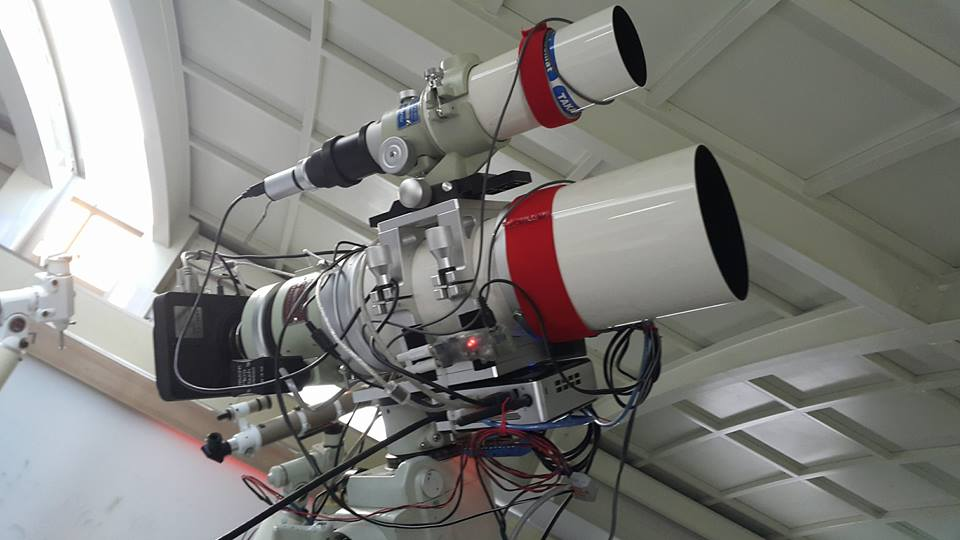
\includegraphics[width=0.8\linewidth]{observing_system}
	\caption{Telescope system for astrophotography}
	\label{fig:observing_system}
\end{center}
\end{figure}

광학계에 의한 별의 상이 검출기에 정확하게 맺히도록 하기 위해서는 포커서를 정밀하게 움직여야 한다. 사진 촬영을 위한 고성능의 광학계는 포커서(Focuser)를 견고하게 만들 뿐 아니라 포커서 노브에 미동 장치가 있어 정밀하게 초점 조절이 가능하다. 하지만 포커서를 조절하기 위해 손을 가져다 대기만 해도 그 진동이 상에 영향을 미치기 때문에 손으로 초점을 조절하는 

사천체를 관측할 때 초점을 맞춘다면 관측할 천체의 모습이 더 선명하게 보인다. 일반적으로 대부분 망원경은 초점을 손으로 맞출 수 있게 설계되어있다. 천체망원경으로 사진 관측을 할 때 정확한 초점 조절은 사진의 품질에 영향을 미치는 요소 중의 하나이다. 초점 조정 시 어려운 점은 초점을 조정하기 위해 초점 조절 노브에 손이 닿으면 진동이 발생하고, 그 진동이 사진의 품질에 영향을 준다. 또한, 초점을 조절할 때 손으로 돌리는 것은 미세한 조정에는 어려움이 있다. 또한, 초점이 완벽하게 맞지 않았는데도 이러한 사진을 찍기 위해서 초점을 맞추는데 많은 시간을 투자해야 한다. 이렇듯 사진을 통하여 정밀한 천체의 사진이 필요한 경우 사람의 손으로는 무리가 있다. 하지만 모터 초점 조절 장치가 있다면 손으로 초점을 맞추는 것보다 정확하게 초점을 맞출 수 있게 된다. 

The present invention provides a temperature compensating focuser and method for use with a telescope having a focus which changes with ambient temperature. \cite{persha2001temperature}
\begin{figure}[h]
	\begin{subfigure}{0.5\textwidth}
		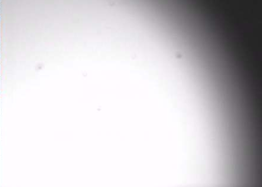
\includegraphics[width=0.9\linewidth, height=5cm]{before} 
		\caption{초점 맞추기 전}
		\label{fig:before}
	\end{subfigure}
	\begin{subfigure}{0.5\textwidth}
		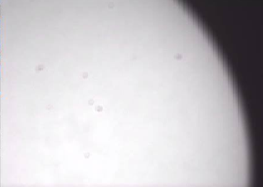
\includegraphics[width=0.9\linewidth, height=5cm]{after}
		\caption{초점 맞춘 후}
		\label{fig:after}
	\end{subfigure}
	\caption{초점을 맞추기 전과 후 비교}
	\label{fig:image1}
\end{figure}






Fig.1.(a), Fig.1.(b)에서 알 수 있듯이 모터 초점 조절 장치를 이용하여 초점을 맞추면 아무것도 하지 않고 그냥 관측했을 때에 비해서 훨씬 정확하게 천체를 관측할 수 있게 된다. Fig.1.(a)와 Fig.1.(b)를 비교하여 보면 Fig.1.(b)의 표면이 훨씬 더 선명하다는 사실을 알 수 있다. 하지만, 모터를 이용하여 초점을 맞춘다고 해도 우리 눈으로 초점을 맞추는 것이기 때문에 정확하지 않을 수 있다. 이러한 문제를 해결하기 위하여 만들어진 자동 초점 조절 장치가 있다. 자동 초점 조절 장치가 현재 개발된 제품이 미국 Starizona 회사의 Micro Touch이다. 이 제품은 자동 초점 조절 시스템이 구현이 잘 되어 있으나, 가격이 499달러로 부담 이 있을 수 있다. 또한, 실제로 모터 초점 조절 장치와 연계해 초점을 맞춰주는 다른 Software도 몇 종류가 있으나 오류가 발생하는 경우가 있다. 따라서 천체망원경의 모터 초점 조절 장치의 컨트롤러 구동 시스템을 개발하면 여러 천체를 관측하는 데 있어서 보다 정확한 사진들을 얻을 수 있을 것이다.

%\begin{wrapfigure}{l}{0.3\textwidth}
%	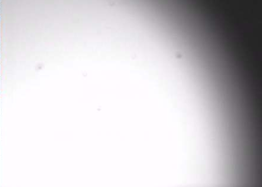
\includegraphics[width=1\linewidth]{before}
%	\caption{초점 맞추기 전}
%	\label{fig:before}
%\end{wrapfigure}

\subsection{연구 목적}

본 논문에서 제안된 방법은 사람이 손으로 제어하는 것보다 정밀하고 빠르게 천체망원경의 초점을 맞출 수 있도록 편의성을 제공하기 위한 기반을 제공하기 위함이다. 이 연구는 Arduino를 이용하여 천체망원경을 이용한 천체관측을 시행할 때 필요한 모터 초점 조절 장치를 조정할 수 있는 모터 초점 조절 장치 컨트롤러 구동 시스템을 구현하고, 초점을 조정하는 알고리즘을 만들어서 천체의 초점을 맞출 수 있도록 한다. 그리고 이와 통신을 할 수 있는 시스템도 개발하여 편의성을 늘리고, ASCOM 드라이버를 제작하여 컴퓨터와의 통신을 가능하게 하는 것이 이 연구의 목표이다.
 % body1
	\section{이론적 배경}

\subsection{천체 관측 시스템}



Figure \ref{fig:telescope} 가 바로 Micro Touch로, 시중에 나와 있는 모터 초점 조절 장치이다. 이를 옆의 컴퓨터와 연결하여 컴퓨터에서도 ASCOM이라는 프로그램을 이용하여 원격으로 모터의 초점을 맞출 수 있도록 설정할 
\begin{wrapfigure}{l}{0.25\textwidth}
	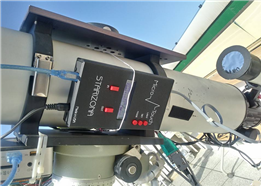
\includegraphics[width=1\linewidth]{telescope1}
	\caption{Micro Touch가 달린 천체망원경}
	\label{fig:telescope1}
\end{wrapfigure}
수가 있다. Fig.2에서 나온 위의 두 버튼(IN, OUT)은 각각 초점을 맞추기 위해 망원경의 길이를 줄이거나 늘일 수 있는 버튼이다. Micro Touch를 수동 혹은 자동으로 작동시켜 IN 또는 OUT의 명령을 내렸을 경우, 모터 초점 조절 장치가 작동하게 된다. 이 모터 초점 조절 장치는 모터를 움직여 천체망원경의 경통의 길이를 조절할 수 있도록 한다. 경통의 길이가 변화하면 그에 따라서 빛이 퍼지는 정도가 달라지므로 이를 잘 조정하면 망원경으로 관측하는 천체의 초점을 맞출 수 있다.

\subsection{Micro Touch와 모터의 조종}

Figure \ref{fig:telescope} 가 바로 Micro Touch로, 시중에 나와 있는 모터 초점 조절 장치이다. 이를 옆의 컴퓨터와 연결하여 컴퓨터에서도 ASCOM이라는 프로그램을 이용하여 원격으로 모터의 초점을 맞출 수 있도록 설정할 
\begin{wrapfigure}{l}{0.25\textwidth}
	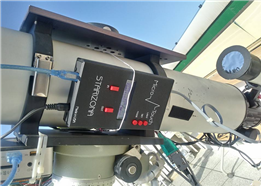
\includegraphics[width=1\linewidth]{telescope1}
	\caption{Micro Touch가 달린 천체망원경}
	\label{fig:telescope1}
\end{wrapfigure}
수가 있다. Fig.2에서 나온 위의 두 버튼(IN, OUT)은 각각 초점을 맞추기 위해 망원경의 길이를 줄이거나 늘일 수 있는 버튼이다. Micro Touch를 수동 혹은 자동으로 작동시켜 IN 또는 OUT의 명령을 내렸을 경우, 모터 초점 조절 장치가 작동하게 된다. 이 모터 초점 조절 장치는 모터를 움직여 천체망원경의 경통의 길이를 조절할 수 있도록 한다. 경통의 길이가 변화하면 그에 따라서 빛이 퍼지는 정도가 달라지므로 이를 잘 조정하면 망원경으로 관측하는 천체의 초점을 맞출 수 있다.

\subsection{온습도 감지기를 이용한 온도 및 습도의 측정}

\begin{wrapfigure}{l}{0.05\textwidth}
	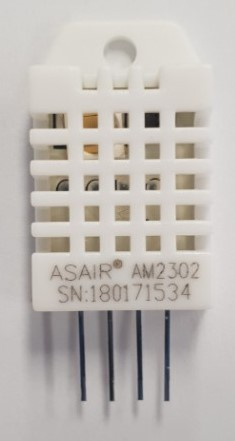
\includegraphics[width=1\linewidth]{DHT22}
	\caption{DHT22}
	\label{fig:DHT22}
\end{wrapfigure}
이 연구를 진행하는 데 Arduino를 사용하는 것이 가장 기본이라고 판단하였기 때문에 Arduino로 실행할 수 있는 것 중 쉬운 축이라고 생각되는 온습도 감지기(DHT22)를 활용하여 온습도를 측정하는 일이었다. 기판을 짜고 코드를 입력하면 Serial Monitor에 온도와 습도가 delay 함수에서 지정한 만큼의 간격을 두고 계속 출력된다. 이를 응용하여 OLED(OLED1306)에 온도와 습도를 실시간으로 출력하는 프로그램을 만들 수도 있다.

\subsection{스테핑 모터}

\subsubsection{스테핑 모터의 종류}

스테핑 모터의 종류는 크게 bipolar와 unipolar 타입으로 나눌 수 있다. 하나는 2상 6선식이라고 불리는 bipolar 스테핑 모터로, 전선이 6개가 연결되어 있다. 2상 4선식이라고도 불리는 unipolar 타입은 전선이 4개가 연결된 모터로, 구동 방식은 bipolar 타입과 크게 다르지 않다.\\
본 논문에서 사용된 스테핑 모터는 2상 6선식 모터이지만, 그 구동 방식이 비슷하므로 bipolar 스테핑 모터에서 필요 없는 2번 선과 5번 선을 제거하는 것으로 bipolar 스테핑 모터를 unipolar 스테핑 모터처럼 구동할 수 있다.

\subsubsection{스테핑 모터의 작동 원리}

\begin{wrapfigure}{l}{0.5\textwidth}
	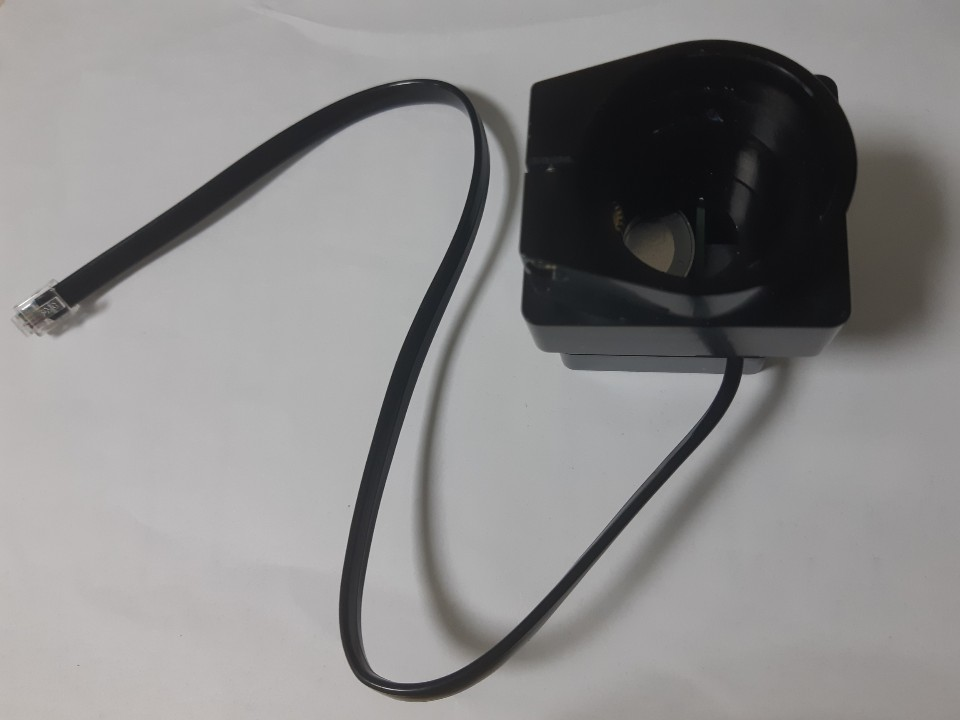
\includegraphics[width=1\linewidth]{stepmotor}
	\caption{스테핑 모터}
	\label{fig:stepmotor}
\end{wrapfigure}
우리가 실생활에서 볼 수 있는 모터 대부분은, 예를 들어 선풍기의 모터는, DC모터이다. DC모터는 전류가 흐르는 상태에서는 계속 회전하기 때문에 원하는 위치에서 멈추는 것이 어렵다. 하지만 스테핑 모터는 회전자 주위에 여러 고정자가 존재하여, 이 고정자들에 흐르는 전류의 변화량에 따라서 회전자 내부의 자석을 회전시키기 때문에, 전류의 양에 따라서 일정한 각도를 정확하게 회전시킬 수 있다. 따라서 본 연구와 같이 회전시키는 것이 중심이 아닌, 정확하게 얼마나 돌아갔는지(어느 각도만큼 돌아갔는지가 중요하게 작용할 때) 대부분 스테핑 모터를 활용하고는 한다. 이렇듯 선별로 흐르는 전류의 양에 의해 회전하는 정도와 속도를 결정할 수 있기에 흔히 ‘마이크로 스테핑’을 이용하여 전류를 여러 단계로 나누어 흘려보내어 더 정밀하게 모터를 제어하는 방법들도 존재한다. 대부분의 스테핑 모터는 1 스텝당(full step) 1.8도를 돈다고 알려져 있다.

\subsection{자동초점조절 알고리즘 및 관련 논문 고찰}

이덕규 외(2014)는 복합재 광구조체와 결합하여 전자광학카메라의 영상 품질을 향상시킬 수 있는 초점 조절 장치를 개발하였다.\cite{leedukgu2014}\\
윤종환 외(2011)는 선명도에 관한 기울기를 이용하여 초점이 맞았는지를 확인하는 방법을 사용하였다.\cite{yunjonghwan2011lcd}\\
박석휘 외(2009)는 모바일 폰용 자동 초점 조절 알고리즘을 초점 값 계산 알고리즘을 이용하여 구현하였다.\cite{parksukhui2009Median}\\
이성희 외(1998)는 각 화소들의 미디언 값의 차이를 이용하여 초점을 맞추는 알고리즘을 구현하였다.\cite{leeseonghee1998Median}
 % 이론적 배경
	\section{연구 과정}

\subsection{하드웨어 제작}

\subsubsection{사용한 부품}

%%박기현샘 선정한 부품들의 특징은 무엇이며 왜 아래 부품들을 선정하였는지 추가할 것

천체망원경 모터 초점 조절 장치 컨트롤러를 제작하기 위해서 필요한 부품들을 선정하였다. 각각의 부품의 특징과 스펙을 아래에 정리하였다. 

\begin{description}[font=$\bullet$~\normalfont\scshape\color{red!50!black}]
	\item [ARDUINO NANO] 모터 초점 조절 장치 컨트롤러를 만드는 데 있어 가장 중요한 부품으로, 일종의 작은 컴퓨터와 같은 역할을 한다. Arduino는 마이크로 컨트롤러를 달고 있는 기판으로, Arduino의 여러 가지 핀에 전선을 연결한 뒤에 코딩하여 Arduino에 올리면 Arduino가 코딩된 내용을 그대로 실행할 수 있도록 하는 hardware이다. 내부에 컴퓨터 역할을 하는 MPU인 ATmega328가 탑재되어 있으며, 5V를 공급할 시에 작동한다. 크기는 45mm x 18mm이다.
	\item [0.96" oled screen I2C] Arduino와 I2C 방법으로 통신을 할 수 있는 OLED 스크린이다. 여러 가지 정보가 전달되며, 모터를 얼마나 돌릴 것인지, 혹은 얼마나 돌려져 있는지 등이 표현될 수 있다.
	\item [DHT22] 온도와 습도를 측정할 수 있는 감지기로, -40~80℃의 넓은 온도 측정범위와 약 0.5℃밖에 없는 오차를 가지고 있다. 이를 통해 온도나, 렌즈의 온도 상태를 볼 수 있으며, 이를 사용하면 좀 더 정밀한 측정이 가능할 것이다.
	\item [Apem MJTP1230B 버튼스위치] 누르는 버튼의 일종으로, 다리가 4개 달린 상태에서 같은 방향에 있는 2개의 전선이 연결된 방식의 버튼이다. 내부의 pull-up 저항을 활용하면 Arduino와 직접 연결하는 것으로 작동시킬 수 있다.
	\item [BP5277-90] 모터를 돌리기 위해서는 12V의 전압이 필요하다. 즉, 12V의 전압을 이용하여 모터를 돌리면서 Arduino를 실행시키기 위해서는 12V를 Arduino의 입력전압인 5V까지 낮출 필요가 있다. 이에 regulator와 축전기를 활용하여 가장 안전하게 5V까지 전압을 낮출 수 있는 regulator를 선택하였다.
	\item [HC-06 bluetooth] 무선통신 장치이다. 여러 가지 무선통신 장치 중에서 블루투스 module의 역할을 하고 있다.
	\item [LED 3mm 90', Ohmite OD473JE] 전원이 여러 개가 존재할 수 있으므로, 모터가 돌아갈 수 있는 전압인 12V의 외부전압이 들어왔을 때만 LED가 깜빡일 수 있게 하여 모터가 돌아갈 수 있는 전압이 되었는지 확인할 수 있도록 하는 역할을 하고 있다.
	\item [Panasonic EEA-GA1C100H] 모터를 돌리는 상황에서 큰 전류를 사용하기 때문에 전류가 역방향으로 흐르는 등의 문제를 방지하기 위하여 100μF의 축전기를 사용하였다.
	\item [SparkFun WRL-13678 (ESP8266, ESP01)] 무선통신 장치이다. 여러 가지 무선통신 장치 중에서 WIFI 모듈을 담당한다. 입력전압이 5V가 아닌 3.3V이다.
	\item [Sprague 1C10X7R104K050B] 부품별로 각각 연결된 축전기로, 모두 같은 전압 차를 가지고 있지만, 전류의 noise filtering을 하는 역할로, 필수적으로 사용되었다.
	\item [TMC2100 (DRV8825)] 스테핑 모터를 돌리는 데 있어서 전류를 쉽게 조절할 수 있게 해주는 module이다. 이뿐만이 아니라 모터를 좀 더 세밀하게 돌릴 수 있게 해주는(스텝 당 돌아가는 각도를 줄여주는) 마이크로 스텝을 구현 가능한데, DRV8825의 핀 중 M1, M2, M3의 up, down을 조절하여 full step을 원래 각도와 비교하면 얼마나 적게 돌릴 것인지 결정할 수 있게 한다. 본 모델은 최대 1/32까지의 마이크로 스텝이 가능하다.
	\item [TE Connectivity/AMP 5525258-3 및 Wurth Elektronik 694106301002] 12V 외부전원과 모터를 연결하는 선을 연결할 수 있게 하는 module이다.
\end{description}

\subsubsection{프로토타입(Prototype) 기판 제작}

주어진 부품들을 하나하나 연결하여 만능기판에 와이어로 납땜을 하여 Figure \ref{fig:prototype}\과 같은 프로토 타입을 회로를 제작하였다. 부품의 갯수가 많아지면서 배선을 하는데 어려움이 있었지만 회로가 정상적으로 동작하는 것을 확인할 수 있었고, 모터 회전, OLED 디스플레이, 시리얼 통신 등의 코드를 연습할 수 있었다.

\begin{figure}[h]
	\begin{center}
		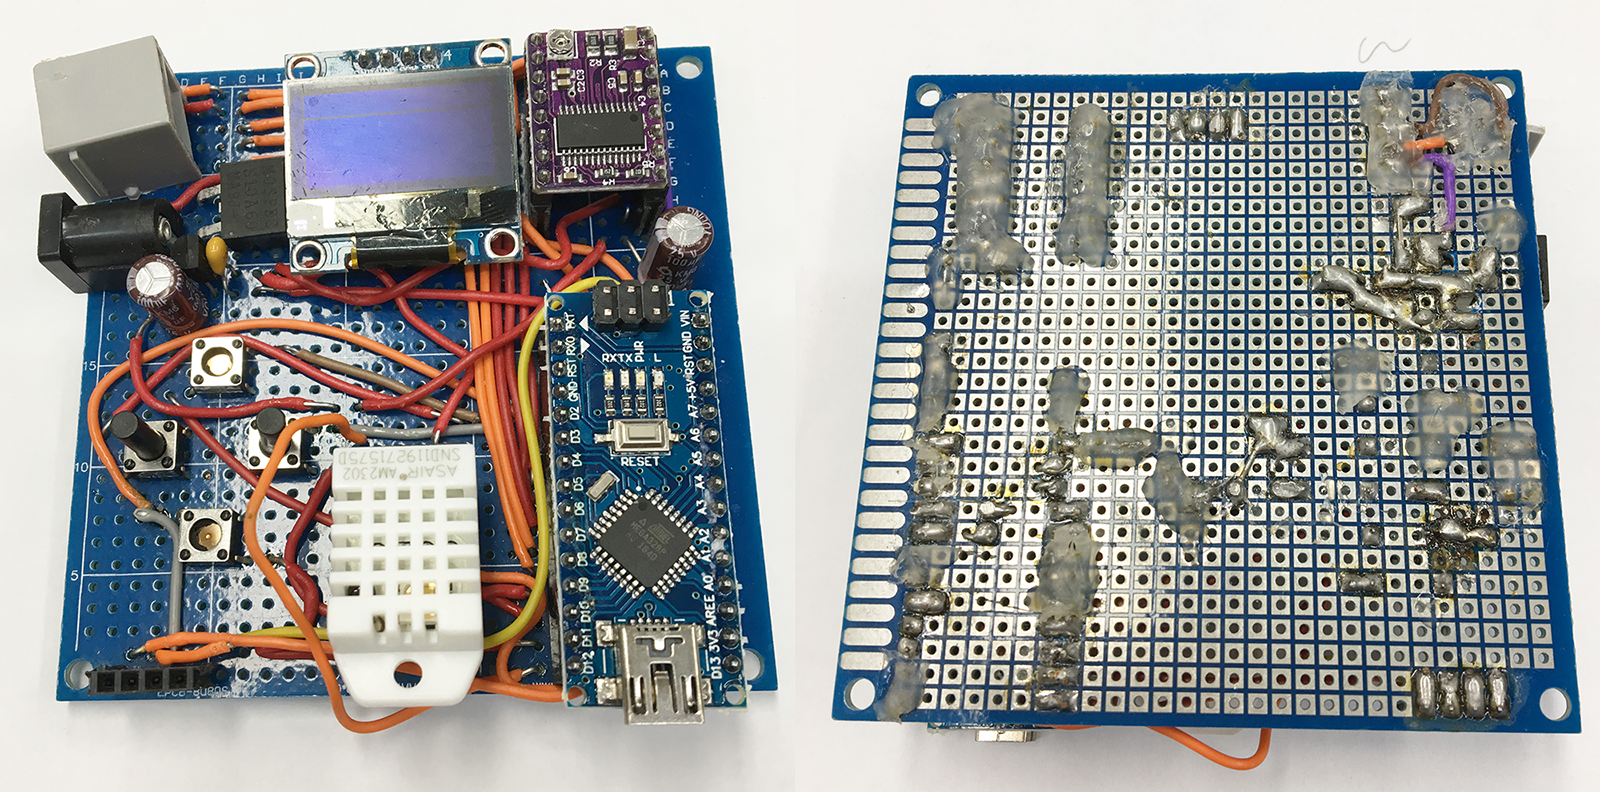
\includegraphics[width=0.9\linewidth]{prototype} 
		\caption{prototype}
		\label{fig:prototype}
	\end{center}
\end{figure}


\subsubsection{회로도 작성}

Circuitmaker 프로그램의 사용법을 숙지하는 데 오랜 시간이 걸렸기 때문에, 그사이에 진행된 연구에서는 만능기판에 여러 가지 부품들을 전선으로 연결하여 사용하는 방법을 택하였고, 연구가 진행되어 만능기판이 복잡해짐에 따라서 여러 프로그램의 도움을 받게 되었다.

연구 초기과정에서는 Arduino와 직접 연동이 가능한 ‘Fritzing’이라는 프로그램을 사용하였지만, 연구가 진행될수록 다른 부품들과 실제로 구현이 가능한 PCB 회로기판을 만들 수 있어야 했기 때문에 보편화한 PCB 회로제작 프로그램이면서 ‘협업’ 기능을 이용하여 동시에 수정이 가능한 ‘Circuitmaker’라는 프로그램을 사용하게 되었다.

각 부품을 사용할 때에는 각 부품의 허용 전류와 같은 여러 가지 특징들을 생각하여 회로를 배선해야 한다. 예를 들어 WIFI 모듈인 ESP8266과 같은 경우 그 입력전압이 Arduino의 출력 전압인 5V가 아닌 3.3V이기 때문에 주의하여야 한다. 또한, 각 부품의 칩별로 제조한 회사의 data sheet를 참조하여 부품을 사용하면서 여러 가지 문제점들을 미리 방지하였다.\\
특히 5V를 3.3V로 바꾸는 과정에서는 전압 나눔 회로를 이용하여 전압을 나눌 수 있으나, 12V를 5V로 바꾸는 과정에서는 전류를 제어하는 것이 필요하므로 부득이하게 regulator를 사용하게 되었다.


Figure \ref{fig:Schematic_Prints}\는 최종 완성한 기판의 회로도이다.
\begin{figure}
	\begin{center}
	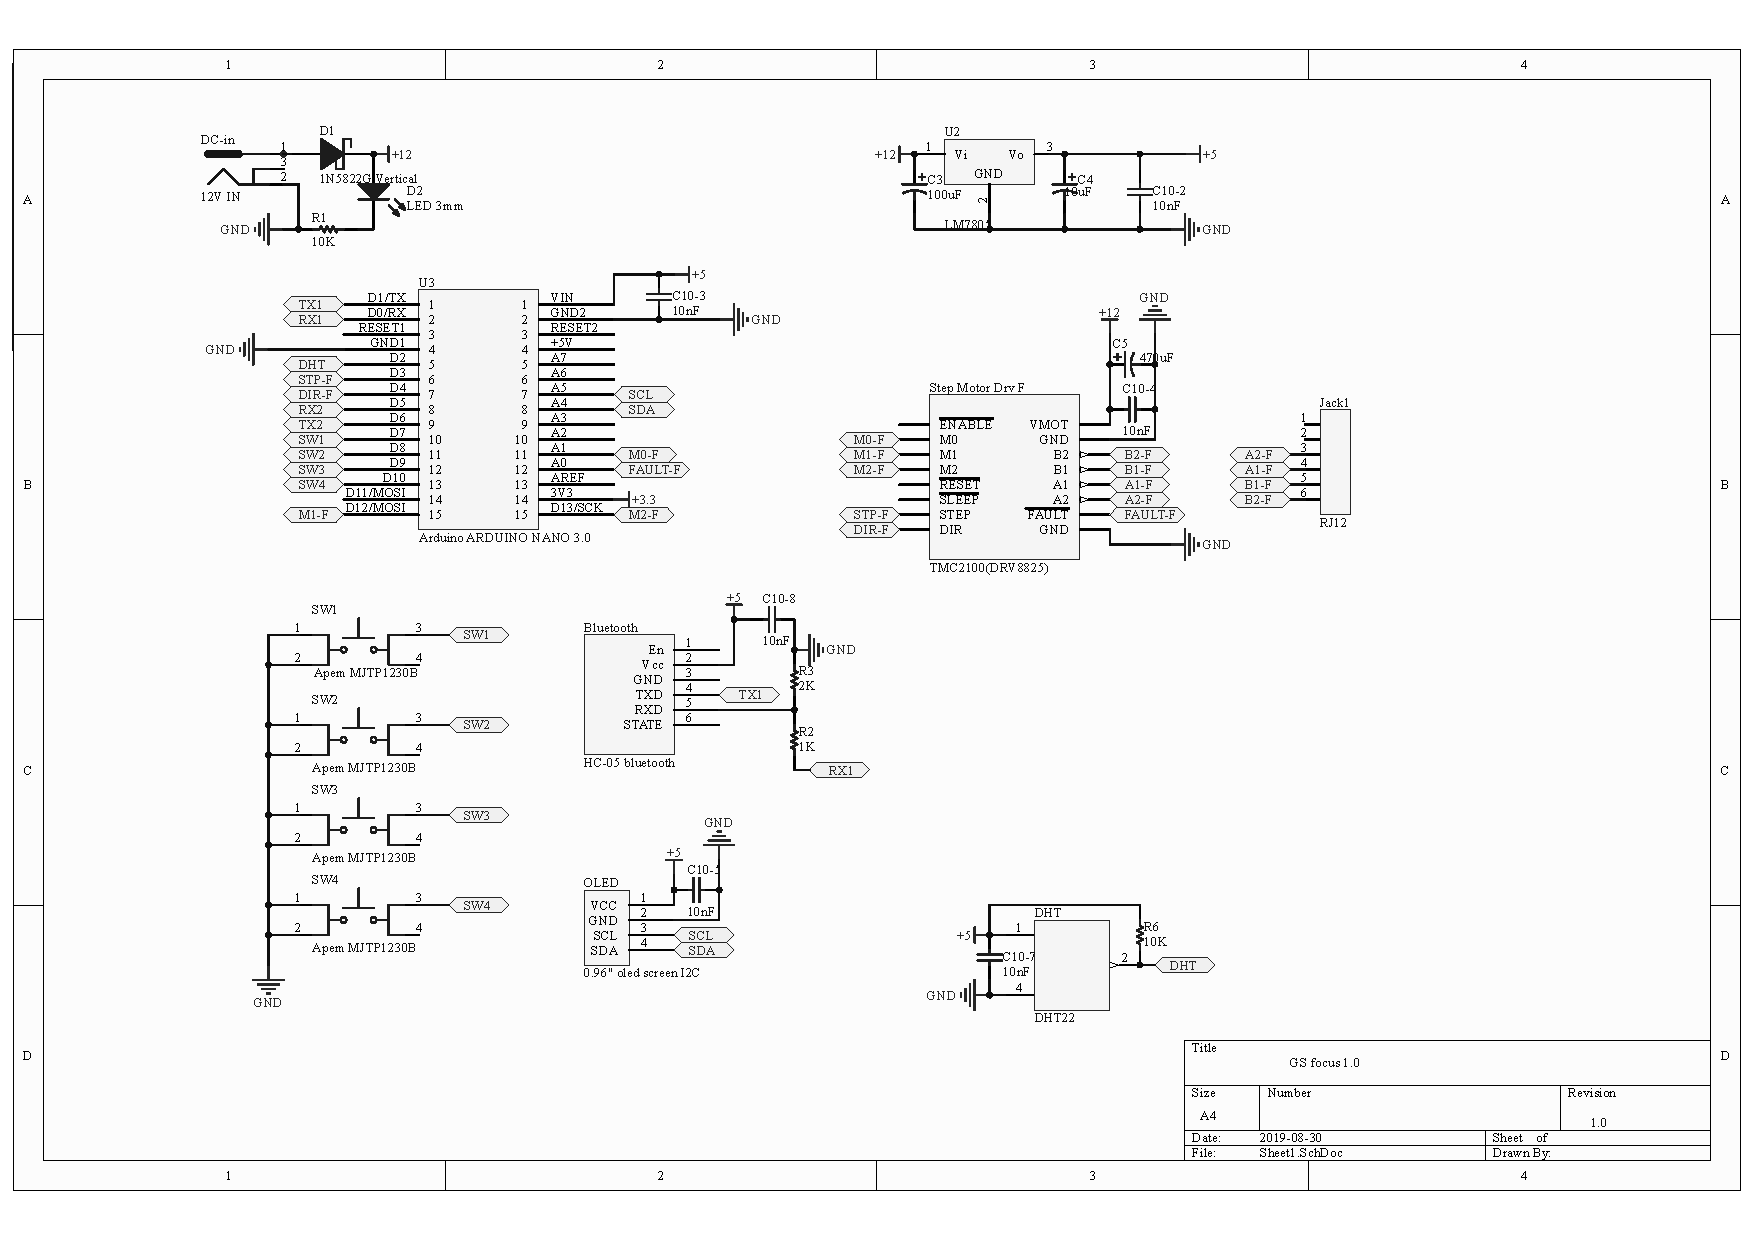
\includegraphics[width=1\linewidth]{Schematic_Prints_color}
	\caption{회로도}
	\label{fig:Schematic_Prints}
	\end{center}
\end{figure}


\subsubsection{기판 제작}
서킷 메이커 프로그램으로 회로를 그린 후 PCB를 디자인 하였다. 

%%박기현 샘  PCB를 디자인하기 위해 와이어링, 부품 배치, 폴리곤 푸어 등을 한 과정을 추가할 것
%%아까 말한데로, 누구나 이 보고서를 보고 따라만들수 있을 정도로 자세하게 적으면 좋겠다.
%%예를 들면 서킷메이커로 작업한 것을 순서대로 기술해 주면 좋겠어..
%% 부품 선정, 와이어링, pcb 제작, 폴리곤 푸어 등등

회로도에 따라 부품들이 와이어로 연결되어 있으므로 적절하게 배치하여 ......    PCB를 제작하였다. Figure \ref{fig:prototype}\은 서킷 메이커로 디자인한 PCB의 삼차원 모습을 나타낸다.

\begin{figure}[h]
	\begin{center}
	\begin{subfigure}{0.45\textwidth}
		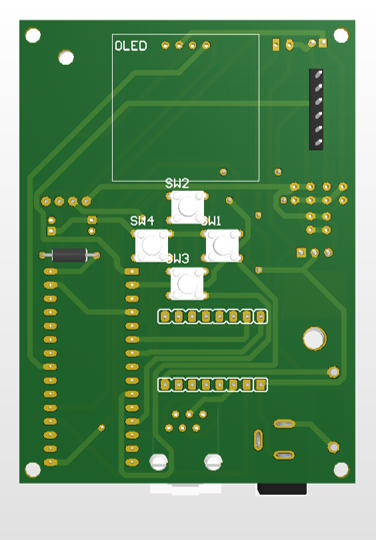
\includegraphics[width=0.9\linewidth]{pcbfront_3d} 
		\caption{Front}
		\label{fig:pcbfront_3d}
	\end{subfigure}
	\begin{subfigure}{0.45\textwidth}
		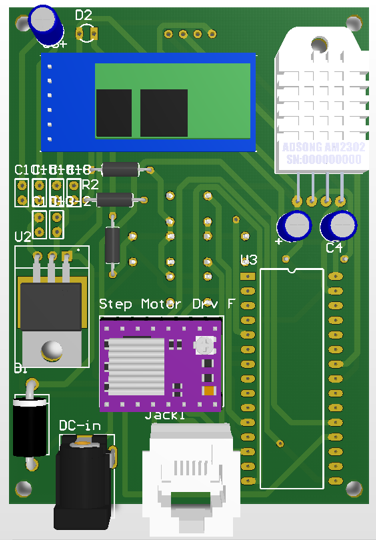
\includegraphics[width=0.9\linewidth]{pcbback_3d}
		\caption{Back}
		\label{fig:pcbback_3d}
	\end{subfigure}
	\caption{Circuit maker로 디자인한 PCB}
	\label{fig:pcb}
	\end{center}
\end{figure}

Figure \ref{fig:pcbcircuit}\은 처음 제작한 PCB Ver. 1 이다. PCB Version 1은 크기가 너무 크게 제작되었다.
\begin{figure}[h]
	\begin{center}
		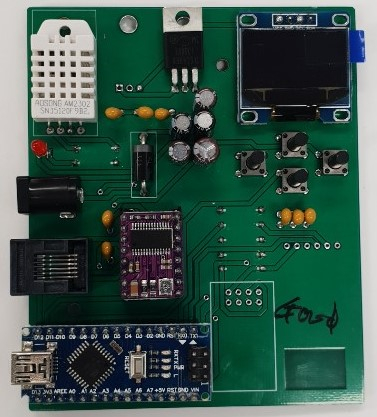
\includegraphics[width=0.6\linewidth]{pcbcircuit}
		\caption{PCB Ver. 1로 완성한 회로}
		\label{fig:pcbcircuit}
	\end{center}
\end{figure}

%%박기현 샘  이후 PCB는 어떤 점을 개선하였는지

\subsection{펌웨어 개발}

%% 아두이노 IDE 실행해서, 어떤 라이브러리를 사용했는지, 라이브러리 설치하는 방법 등을 자세히 기술하면 좋겠다. 
\subsubsection{아두이노 라이브러리}
펌웨어에 필요한 기본적인 기능들을 구현하기 위해서는 연결되어있는 부품들을 컨트롤할 수 있는 방법이 필요했고, 이들을 단순화시켜 함수로 정리한 라이브러리를 사용하여 효율적으로 개발을 진행할 수 있었다.
IDE에서 새로운 라이브러리를 추가하기 위해서는 상단의 도구 창에서 스케치>라이브러리 포함하기>라이브러리 관리 또는 .ZIP 라이브러리 추가...를 선택하여 관련 작업을 진행할 수 있다.\\
본 연구에서 사용한 라이브러리는 다음과 같다.
\begin{description}[font=$\bullet$~\normalfont\scshape\color{red!50!black}]
	\item [AccelStepper.h] 모터의 전반적인 움직임에 있어 필요한 라이브러리다. 스테핑모터를 컨트롤할 수 있도록 하는 기능을 포함하며, 모터의 객체를 생성할 때 스테핑모터 드라이버가 없는 경우는 각각의 핀을 아두이노와 연결하여 객체를 만들 수 있도록 하며, 본 연구와 같이 스테핑모터 드라이버가 있는 경우에는 드라이버의 DIR핀과 STEP핀만을 이용하여 객체를 생성할 수도 있다. 중요한 함수들을 몇가지 나열하자면, \\
	
	
	AccelStepper::currentPosition() : 현재 position에 있는 값을 반환한다.\\
	AccelStepper::setCurrentPosition(int p) : p를 현재 position으로 한다.\\
	AccelStepper::moveTo(int p) : p위치의 position으로 이동한다.\\
	
	
	등이 존재한다. AccelStepper.h 라이브러리의 단점은 그 자체로 microstepping을 지원하지 않기 때문에 이를 바꾸기 위해서는 드라이버를 통해 강제로 바꾸어야하며, 이로 인해 바뀌는 step당 position을 적용시키기 어렵기 때문에 microstepping을 변환하기 위해서는 setCurrentPosition함수가 반드시 동반되어야 한다는 점이다.
	
	\item [DHT.h] DHT22의 컨트롤을 가능하게 하는 라이브러리다. DHT22는 하나의 핀으로 입력과 출력을 모두 하기 때문에 그 방법과 순서만 알면 비교적 쉽게 함수가 제작이 가능하다. DHT22로 온도와 습도를 입력받을 때 걸리는 시간(약 2초당 한번)을 계산하여 펌웨어를 개발하는 것이 좋다.
	
	\item [Adafruit\_SSD1306.h] 본 연구에서 사용된 OLED인 SSD1306을 컨트롤하기 위해 필요한 라이브러리로, 보통 Adafruit\_GFX.h와 Wire.h를 함께 사용하게 된다. SSD1306은 I2C 통신을 사용하므로 복잡한 통신을 이용하기 위해서는 다른 라이브러리들 또한 포함시켜야 할 것이다. 이 라이브러리는 업로드 속도가 빠르고 한번에 모든 화면을 바꿀 수 있다는 장점이 있지만, 사용할 수 있는 폰트가 정해져 있고 아두이노의 자체 메모리를 아주 많이 잡아먹는다는 단점이 있다.
	
	\item [U8glib.h] 많은 종류의 OLED를 컨트롤할 수 있도록 개발된 라이브러리로, 지원하는 OLED 중 SSD1306또한 포함되어 있다. Adafruit\_SSD1306.h와는 다르게 지원하는 폰트와 그 크기가 비교적 자유로우며, 아두이노의 자체 메모리를 작게 잡아먹으며 한번에 작성하지 않는다는 특징이 있지만 업로드 시 많은 시간이 소요된다는 단점도 존재한다.
\end{description}

\subsubsection{serialPort 통신}
펌웨어를 개발할 때 필요한 중요한 기능 중 하나는 컴퓨터와 통신이 가능해야 한다는 것이다. 아두이노는 UART 시리얼 통신을 사용하는 데, 직렬 통신을 사용하기 때문에 그 속도는 떨어질 수 있어도 더 먼 거리를 보낼 수 있다는 장점이 있으며, UART방식을 사용하기 때문에 정해진 BaudRate로만 통신이 가능하다. 아두이노의 0번 핀(RX: Receive Data)이 컴퓨터에서 보내는 신호를 받고, 1번 핀(TX: Transmit Data)으로 신호를 보내게 되며, 이들은 USB 케이블을 통해 컴퓨터와 직접적으로 연결된다.

아두이노 IDE 상에서는 우측 상단의 돋보기 모양의 아이콘을 클릭함으로써 시리얼 모니터를 실행할 수 있다. 시리얼 통신을 이용하기 위해서는 지정된 BaudRate로 COM Port를 열어야한다. 따라서 코드 중에 반드시 시리얼 포트를 여는 코드가 있어야 하며, 이후 수신된 값을 활용할 수 있는 기법들을 이용해 데이터를 사용할 수 있도록 한다. 주로 사용되는 함수는 다음과 같다.

\begin{description}[font=$\bullet$~\normalfont\scshape\color{red!50!black}]
	\item [Serial.begin(int BaudRate)] 지정된 BaudRate로 시리얼 통신을 시작한다.
	\item [Serial.print(String s)] String형 변수 s의 값을 컴퓨터로 송신한다. 비슷한 함수로 Serial.println(String s)가 있는 데, 이는 값을 수신한 이후 줄을 띄게 한다.
	\item [Serial.available()] 시리얼 통신이 진행되고 있는지를 bool 형태로 반환한다. 이를 응용하면 다음과 같은 예제로 수신된 String을 미리 선언된 inputString에 저장할 수 있다.
	%%P_serialEvent사진 첨부
\end{description}


\subsection{ASCOM driver 개발}

%% 아스콤 드라이버를 개발하기 위해서 ASCOM faltfrom을 설치하고, 개발자 예제를 설치하고, 
%%visual studio 2017을 설치하고, 템플릿 불러온 후, 어떤 부분을 수정해서 만들었는지 자세히 기술.

%% 펌웨어와 ASCOM 간에 통신 프로토콜은 무엇으로 정했는지, 컴퓨터에서 어떤 명령을 주면 어떻게 동작하는지 등등


모터 초점 조절 장치를 활용하기 위해서는 별의 크기를 분석해서 돌려야 하므로 컴퓨터와의 연동을 위하여 초점 조절 장치의 ASCOM 드라이버를 C\# 코딩을 이용하여 제작한다. ASCOM 드라이버를 이용하면 카메라로부터 정보를 컴퓨터가 받아서 데이터를 분석하고, 이 분석한 데이터를 이용하여 모터를 어떻게 조절해야 할지 명령을 내리면 ASCOM 드라이버를 통해 정보를 전달하여 모터를 제어한 대로 조절이 가능하다.


현재 우리가 사용하는 프로그램은 ASCOM에서 만든 프로그램이고, ASCOM의 프로그램 대부분은 그 회사만의 표준 Protocol을 사용한다. 따라서 우리가 만드는 모터 초점 조절 장치 컨트롤러를 ASCOM Protocol에 따라 정보를 전달할 수 있도록 하면 일반 컴퓨터에 있는 ASCOM 프로그램을 이용하여 우리가 제작한 모터 초점 조절 장치 컨트롤러를 사용할 수 있도록 하는 것이 핵심이라고 할 수 있다.





 % 원래 있던 문
	\section{결과 및 토의}

본 연구에서는 Fig. \ref{fig:How_it_works_big}\과 같이 천체 망원경 모터 포커서 컨트롤러를 구동하기 위한 회로를 제작한 후 ASCOM 프로토콜에 호환되도록 펌웨어를 제작하였고, ASCOM 드라이버를 개발하여 ASCOM을 지원하는 소프트웨어로 구동하는데 성공하였다.

\begin{figure}[h]
	\begin{center}
		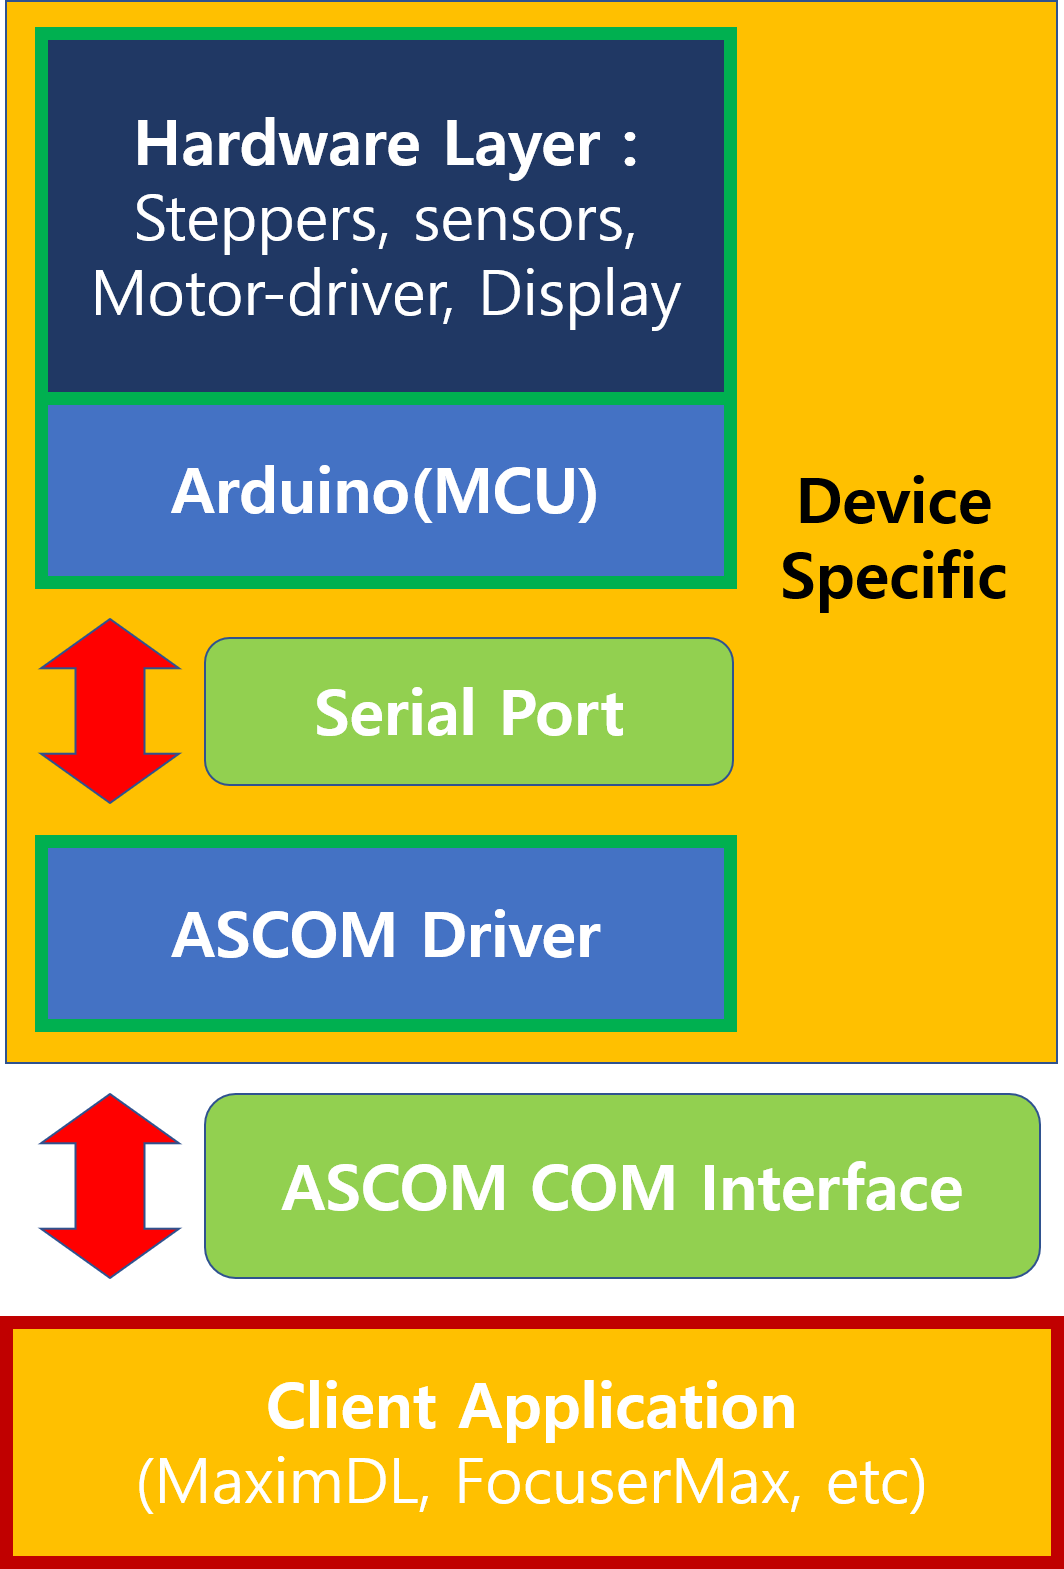
\includegraphics[width=0.4\linewidth]{How_it_works_big}
		\caption{동작 원리}
		\label{fig:How_it_works_big}
	\end{center}
\end{figure}

\subsection{모터 초점 조절 장치 컨트롤러 및 펌웨어}

펌웨어는 컴퓨터와 다르게 지정된 디스플레이에만 표시를 할 수 있다는 특징이 있다. 따라서 여러가지 기능이 존재하더라도 한번에 여러가지의 동작을 진행할 수는 없다. 그렇기 때문에 모터에 내려야 하는 여러 명령들을 효율적으로 처리하기 위해, 하드웨어에 탑재된 버튼을 이용하여 이동과 선택이 쉬운 메뉴와 서브메뉴를 만들어 사용하는 방식을 택하여 핵심 기능들이 모두 펌웨어에 들어갈 수 있도록 하였다.

펌웨어의 첫 번째 기능은 모터 초점 조절 장치의 핵심이라고도 할 수 있는 기능으로, 앞서 설명하였듯이 스테핑 모터를 조절하는 데 있어 가장 중요한 것은 정확한 스텝으로 정확한 각도를 이동하는 것이다. 즉, 제작한 펌웨어에는 현재 스테핑 모터의 각도를 나타내는 정보(position)를 나타낼 수 있으며, 버튼을 이용하여 아주 작은 간격(single step)으로 모터의 각도를 이동할 수 있도록 하였다.
ㅂ
장치를 사용하다보면 제공되는 최대 스텝수가 부족하거나 현재 위치를 기억해야 할 때가 있다. 이럴 때 필요한 기능이 position을 원하는 곳으로 초기화하는 것이다. 예를 들어, 대부분의 사람들은 포커서가 끝에 위치할 때의 position을 0으로 설정하고 싶을 것이다. 꼭 끝점이 아니더라도 이미 초점을 맞춘 상황을 기준으로 삼고 싶어서 position을 바꾸고 싶을 수 있을 것이다. 이 때 필요한 기능이 position을 지정된 범위 내에서 초기화시키는 것(reset position)이다. 위에서 설명한 상황이 아니더라도 focuser을 껏다가 위치를 이동시켰던 경우에도 실제 위치를 기억하지 못할 때도 있을 것이다. 이런 상황에서도 position을 초기화시키는 기능이 사용될 것이다.

부가적인 기능으로, 망원경의 특성의 차이때문에 같은 각도를 이동하더라도 포커서가 이동하는 거리가 달라질 수도 있고, 필요한 힘이 달라지거나 한번에 이동하는 거리가 달라질 수도 있다. 이렇게 필요한 상황에 따라서 적절하게 microstepping을 바꿀 수 있는 기능또한 펌웨어에 탑재되어있다. 또한, 모터를 움직이는 상황이 아니라면 센서에서 측정된 온도와 습도를 표시할 수 있도록 하였다.

\subsection{ASCOM 드라이버 개발}

ASCOM 드라이버를 ASCOM Protocol에 맞게 개발하여 여러가지 프로그램 및 망원경 사이의 편의성을 증대시키고자 하였다. ASCOM 드라이버는 직접 띄우는 창을 설정하여 여러가지 상황에 맞는 기능들을 제공할 수 있으며, 컴퓨터의 화면 상에서 일어나기 때문에 비교적 많은 정보를 한번에 표현할 수 있다.

C\#에서 지원하는 파일 형식은 .cs의 이름을 가지고 있으며, ASCOM Protocol에 맞게 작성된 ASCOM 드라이버를 표현하는 프로젝트는 크게 3가지 부분으로 이루어져 있다. Driver.cs 파일, SetupDialogForm.cs 파일, MainWindow.cs 파일이 그 세 가지이며, 각 파일들에서 실행시키는 영역이 모두 다르게 설계되어있다.

Driver.cs는 serialPort를 이용하여 펌웨어와 직접적으로 통신하는 기능을 가지고 있다. 이 파일을 가장 중요한 기능은 프로그램이 내릴 수 있는 여러가지 명령을 serialcommand를 설정하여 각각 실행할 수 있도록 하는 것이다. 만약 서로 다른 프로그램에서 serialPort를 통한 연결(Port를 open한다고 표현한다)을 진행하려고 하면 그동안 진행했던 정보들을 모두 다시 전달해야하기 때문에 복잡한 처리과정을 거쳐야 한다. 때문에 serialPort와 관련된 함수 및 연결을 하나의 파일에서 모두 실행시킬 수 있도록 하였다.

SetupDialogForm.cs는 ASCOM 드라이버를 선택하는 과정에서 직접적으로 연결을 진행하기 전에(직접적인 연결은 Connect를 눌러야 시작된다) 필요한 설정들을 확인하는 절차이다. 이 파일에서는 드라이버와 펌웨어 사이에 연결되어있는 COM port(serial 통신을 하기 위해 usb로 연결되어 있는 포트)를 지정하며, 모터의 microstepping을 설정한다. microstepping설정을 모터를 움직이는 도중에 직접 설정하게 되면 한 스텝당 이동하는 position이 달라지기 때문에 정확한 거리를 계산할 수 없게 되며, 측정을 한 번 진행할 때마다 Position 사이의 거리가 달라진다. 따라서 직접 연결을 진행하기 전에 microstepping을 다시 확인하게 된다.

MainWindow.cs는 직접 연결을 실행했을 때 우리 눈에 직접 들어오는 컨트롤 창의 정보에 대한 파일이다. MainWindow의 버튼들은 각각 펌웨어에서 설정한 serialcommand와 연결되어있어 버튼이 눌릴 때마다 Driver.cs에서 serialcommand를 통해 자료를 주고받으며, 새로 업데이트된 정보는 다시 MainWindow 창에 표시되는 작업이 반복되게 된다. 

펌웨어보다 자유로운 설정이 가능하기 때문에 보다 많은 기능들을 탑재할 수 있다. 기본적인 기능인 스텝당 움직이는 기능과 더불어 한번에 이동할 single step을 얼마나 크게 할지 직접 설정할 수 있고, 원한다면 모터를 그 상태에서 정지시킬 수도 있으며, 원하는 position을 입력하면 모터가 그 position으로 자동으로 이동하게 할 수도 있다(Move to). 부가적으로는 microstepping과 온도 및 습도를 실시간으로 확인할 수 있으며, 모터가 움직이는 속도와 가속도를 범위 내에서 직접 설정할 수도 있다.

Fig. \ref{fig:focuserchooser}\은 ASCOM에서

\begin{figure}[h]
	\begin{center}
		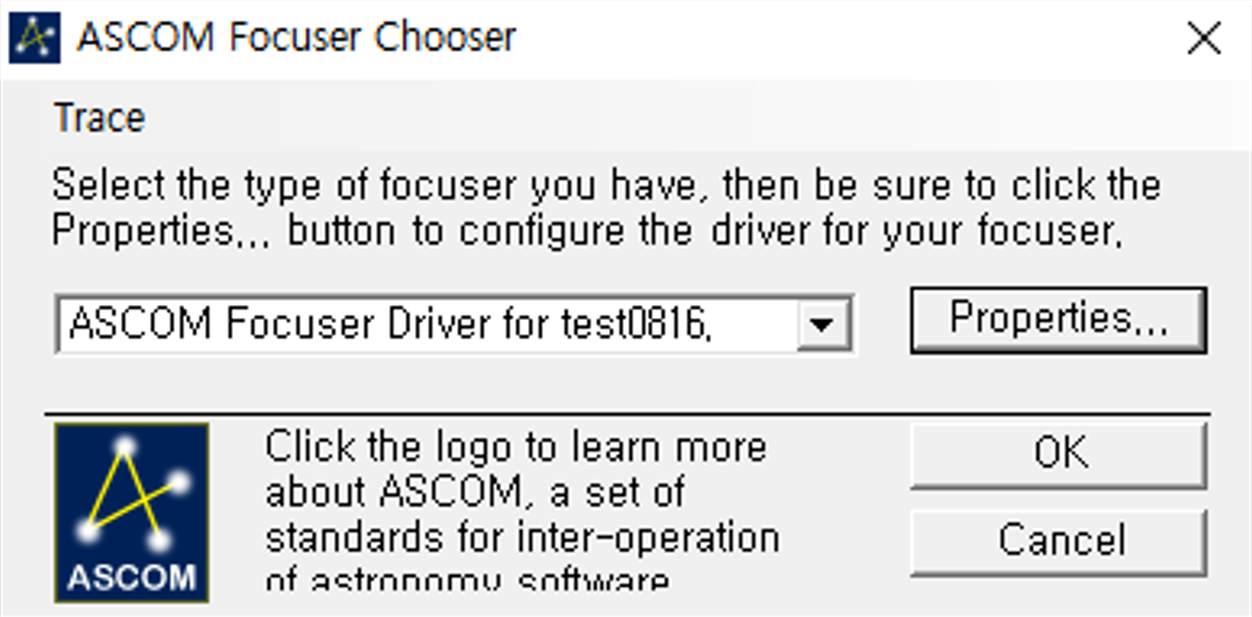
\includegraphics[width=0.6\linewidth]{focuserchooser}
	\end{center}
	\begin{tikzpicture} [remember picture, overlay]
	\node[rectangle, draw, fill=black!10, minimum size=0.5] at (3.3, 3.4) {(a)};
	\node[rectangle, draw, fill=black!10, minimum size=0.5] at (13.4, 3.4) {(b)};
	\node[rectangle, draw, fill=black!10, minimum size=0.5] at (13.4, 2.35) {(c)};
	\node[rectangle, draw, fill=black!10, minimum size=0.5] at (13.4, 1.55) {(d)};
	\end{tikzpicture}
	\caption{Focuser chooser windows : (a)choosing focuser, (b)Properties; excute SetupDialogForm.cs, (c)OK; apply results, (d)Cancel; close Form}
	\label{fig:focuserchooser}	
\end{figure}

\begin{figure}[H]
	\begin{center}
		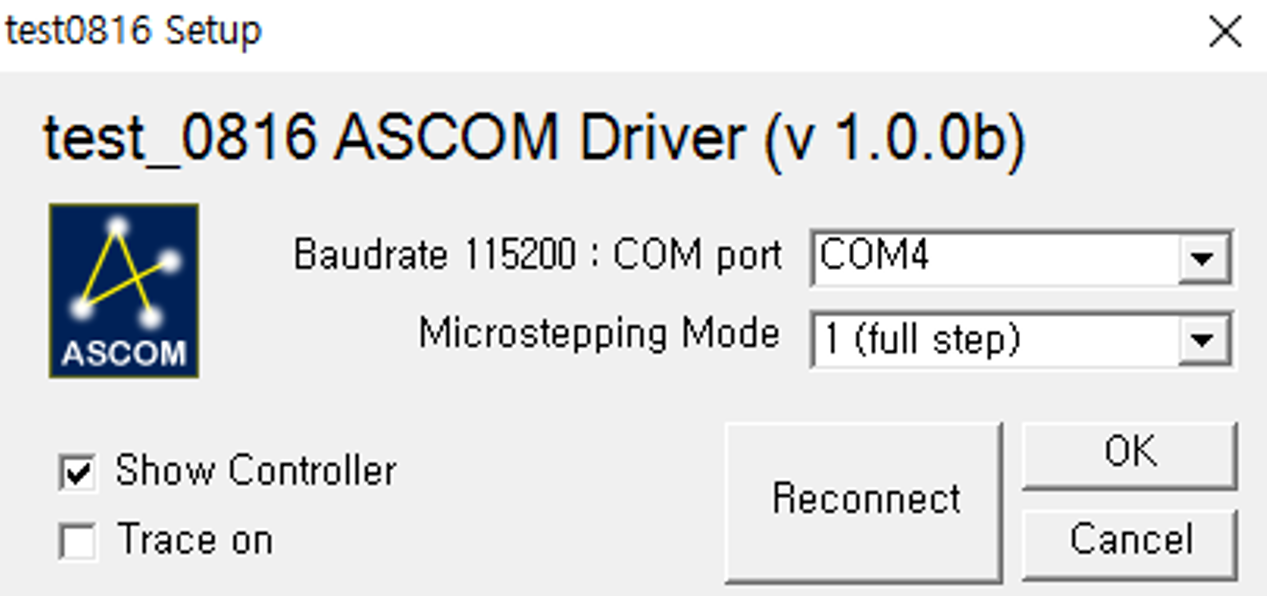
\includegraphics[width=0.6\linewidth]{setupdialogform_capture}
	\end{center}
	\begin{tikzpicture} [remember picture, overlay]
	\node[rectangle, draw, fill=black!10, minimum size=0.5] at (3.3, 1.7) {(a)};
	\node[rectangle, draw, fill=black!10, minimum size=0.5] at (7.4, 3.15) {(b)}
	\node[rectangle, draw, fill=black!10, minimum size=0.5] at (13.4, 3.7) {(c)};
	\node[rectangle, draw, fill=black!10, minimum size=0.5] at (13.4, 3.0) {(d)};
	\node[rectangle, draw, fill=black!10, minimum size=0.5] at (13.4, 2.1) {(e)};
	\node[rectangle, draw, fill=black!10, minimum size=0.5] at (13.4, 1.45) {(f)};
	\end{tikzpicture}
	\caption{SetupDialogForm : (a)basic settings; checked show UI allows to show mainWindow when connected, (b)Reconnect; try to find COM Port, (c)COM Port; find TFocuser, (d)Microstepping; set Microstepping mode, (e)}
	\label{fig:setupdialogform_capture}	
\end{figure}


	\section{결론 및 제언}

\subsection{결론}
	
본 연구를 통하여 천체망원경 모터 포커서 컨트롤러인 GS-touch를 다음과 같이 개발하였다. 

첫째, 아두이노 나노를 기반으로 2상 바이폴라 스테핑 모터 드라이버, OLED 디스플레이어, 온습도 센서 등이 연결된 모터 포커서 컨트롤러인 GS-touch의 하드웨어를 제작하여 구동에 성공하였다. 전원은 DC 12V를 사용하며, 4개의 버튼으로 메뉴를 선택하거나 모터를 정방향 역방향으로 회전시킬 수 있도록 설계하였다.

둘째, GS-touch를 구동할 수 있는 펌웨어을 제작하였다. 펌웨어의 기능은 DRV8825를 이용하여 스테핑 모터를 제어할 수 있도록 하였고, DHT22를 이용하여 온도, 습도 값을 읽어들여 OLED 디스플레이어에 표현할 수 있도록 하였다. 또한 버튼 조작으로 OLED 디스플레이어에 표시되는 메뉴를 조정할 수 있도록 하였다. 

셋째, GS-touch 전용의 ASCOM 드라이버를 개발하여 GS-touch를 PC에 연결하여 ASCOM을 지원하는 MaximDL, FocusMAX 등의 소프트웨어로 구동하는데 성공하였다.

개발된 GS-touch는 기존 제품에 비해 다음과 같은 장점을 가지고 있다. 

첫째, GS-touch는 2상 바이폴라 스텝모터 드라이브인 DRV8825를 사용하여 허용 전류 값이 $3 \textrm{A}$로 micro touch에 비해 월등히 크다. 사진 관측의 경우에는 리듀서, CCD 등 무거운 촬영 장비를 장착하게 되는데 DRV8825의 스펙은 무거운 사진 관측 장비를 장착하고 초점을 조절하는데 무리가 없다. 또한 DRV8825는 1 부터 32 마이크로 스텝까지 펌웨어로 설정 가능하여 포커서의 기어비에 따라 모터 회전 속도를 쉽게 조정할 수 있다. 

둘째, GS-touch는 OLED 디스플레이어를 사용하여 2상 바이폴라 스텝모터 드라이브인 DRV8825본 연구에서 제작된 ASCOM 드라이버의 가장 큰 특징은 직접 개발한 모터제어기를 사용하였기 때문에 그 연동성이 매우 뛰어나다는 것이다. 예를 들어, 모터제어기에 들어있는 마이크로 스텝을 바꾸는 기능은 직접 제작한 ASCOM 드라이버에 그대로 같은 기능을 넣을 수 있었다. 또한 펌웨어에는 없는 기능이더라도 ASCOM 드라이버를 활용하여 더 좋은 활용 방안들을 찾아낼 수 있으며, 

셋째, GS-touch는 DHT22 온습도 센서를 사용하여 온도 뿐 아니라 습도도 파악할 수 있다. 

넷째, GS-touch는 크기가 작아 천체망원경에 장착하기가 용이하다. 

\subsection{제언}

현재 개발된 GS-touch는 초보 단계로서 개선할 수 있는 부분들이 아직 많이 있다. 다음 버전의 하드웨어 부분에서는 버튼 스위치를 좀더 내구성이 좋은 부품으로 교체하는 것이 좋을 것으로 생각된다. 또한 OLED 와 센서의 전원은 아두이노에서 출력되는 전원을 사용하여 외부 전원을 연결하지 않아도 메뉴 조작이 가능하도록 개선할 생각이다.

\begin{description}[font=$\bullet$~\normalfont\scshape\color{red!50!black}]
	\item [Backleash 보정 기능 추가] 모터 포커서를 반대 반향으로 구동할 때 발생할 수 있는 backleash 값을 측정하여 보정할 수 수 있는 기능을 추가할 수 있다.
	\item [MCU 변경] ARDUINO NANO로 펌웨어를 개발할 때 메모리 용량이 작아 어려움을 겪었다. STM32L432KC 같은 는 ARDUINO NANO보다 성능이 좋은 Arduino로, 방향만 반대일 뿐 핀의 순서와 종류가 모두 같아 ARDUINO NANO에 넣었던 펌웨어를 그대로 사용할 수 있다.
	\item [Heating system 추가] 천체 관측시 렌즈에 이슬이 맺혀 관측에 어려움을 겪는 경우가 종종 있다. 이를 해결하기 위하여 날씨가 추운 날에는 모터가 얼어서 돌아가지 않거나 렌즈에 서리가 껴서 초점이 맞아도 맞지 않은 것으로 판단할 수 있다. 따라서 이를 예방하기 위하여 열선을 깔아서 DHT22에서 측정한 온도를 바탕으로 특정한 온도 이하로 내려가게 된다면 열선이 활성화될 수 있게 할 수 있다.
	\item [EEPROM 활용] EEPROM은 Arduino 내부에 저장된 비휘발성 메모리로, 컴퓨터의 ‘RAM’과 같은 역할을 하고 있다. 비휘발성이기 때문에 Arduino를 초기화하거나 껐다가 다시 켰더라도 정보를 저장하고 있다. 
	Arduino별로 한 EEPROM의 주소에 들어갈 수 있는 수의 크기가 달라진다. ARDUINO NANO는 4KB의 EEPROM을 지원하므로 0~255까지의 수를 한 번에 저장할 수 있다. 이렇게 저장할 수 있는 수가 작으므로, 여러 가지 주소를 활용하여 큰 수 또한 나타낼 수 있다.(수를 진법으로 바꾸는 과정과 유사함) 실제로 이를 기반으로 펌웨어를 제작하여 보았지만, 수가 약 32000 이상으로 넘어가는 상황에서는 갑자기 수가 이상하게 커지는 오류가 발견되었고, 이를 고쳐야 할 것이다.
	\item [모터 연결 상태 체크 기능 추가] 모터의 연결 상태는 펌웨어를 실행하는 데 아주 중요하다. 만약 펌웨어가 실행되는 도중에 모터가 연결되지 않으면, 스위치를 움직였을 때 스위치의 숫자는 움직이지만, 모터는 움직이지 않아 결과적으로 숫자의 오류를 불러일으킨다. 또한, 모터를 펌웨어가 실행되는 도중에 연결선을 뽑으면 펌웨어에 에러가 일어나는데, 이 경우 다시 모터를 꽂더라도 정상적으로 실행이 되지 않는다. 따라서 이런 여러 상황에 대하여 모터의 연결 상태를 대비한 에러 코드를 설정해야 숫자와 모터가 오차를 일으키는 일이 없을 것이다.
\end{description}

또한 GS-touch를 활용하여 태양, 행성, 달 등 점 광원이 아닌 천체의 초점 조절 알고리즘을 개발할 생각이다. 앞서 언급한 것처럼 별은 점 광원이므로 FWHM이나 HFD를 이용하여 초점 조절하는 알고리즘이 개발되어 있으나 태양, 행성, 달 등 점 광원이 아닌 천체는 FWHM이나 HDF를 이용한 알고리즘을 적용하기 힘들다. GS-touch를 이용하면 모터 포커서를 정밀하게 제어할 있으므로 태양, 행성, 달 등을 관측할 때 각각의 천체에 적랍한 자동 초점 조절 알고리즘 구현하는데 활용할 수 있을 것으로 생각된다. 

	%\section{추후 연구}

\subsection{카메라(또는 CCD) 제어 Software 개발}

사진 관측을 이용해서 얻은 사진을 컴퓨터로 연결하여 분석이 가능할 수 있도록 만든 카메라(CCD) 제어 시스템을 개발한다. 이렇게 분석한 사진을 컴퓨터로 보낼 수 있어야 한다. 구체적으로 제어 시스템과 관련된 이야기를 하면, 카메라가 별의 크기와 관련된 정보를 분석해야 하는데, 이에는 두 가지 방법이 있다. 첫 번째 방법은 밝기의 기울기 값으로 초점이 맞음을 판단하는 것이다. 즉 수치화된 밝기를 이용하는 것이다. 각 픽셀에는 밝기에 대한 수치적인 정보가 존재한다. 인접한 픽셀의 수치 차이가 크다면 밝기 차이가 큰 것으로, 밝기 기울기가 큰 것이다. 이를 이용한다면 밝기 기울기가 가장 큰 순간이 초점이 맞았을 때로 판단하여 초점을 맞출 수 있을 것이다. 두 번째 방법은 천체의 크기로 초점이 맞음을 판단하는 것이다. 일정 밝기 이상의 픽셀에 대한 분포를 계산하는데, 각각 사진 중 가장 적은 픽셀이 조건을 만족하는 사진을 찾으면 그 사진을 초점이 맞았다고 판단할 수 있을 것이다. 이렇게 초점이 맞았음을 판단하는 것 외에도 카메라에 나오는 화면의 변화를 보아야 하므로 연속적인 변화를 실시간으로 보낼 수 있는 프로그램을 만들어서 컴퓨터가 제대로 인식을 하여 모터에 올바른 명령을 내릴 수 있는지 확인하면 가능하다.

\subsection{자동 초점 조절 알고리즘 구현}

천체망원경의 초점을 맞추기 위해 사진 관측의 사진을 연속적으로 찍어서 컴퓨터로 보내주고, 컴퓨터는 이를 분석하여 초점 조절 장치 컨트롤러에 별의 크기가 커지고 있는지 작아지고 있는지 정보를 알고리즘에 보내준다. 그러면 프로그래밍 된 Arduino가 모터를 어느 방향으로 돌려야 하는지 판단하여 모터를 돌리고, 이 과정을 반복하여 별의 초점이 맞을 때 이 과정을 멈춘다. 이러한 과정이 일어나는지 실제로 천체망원경으로 직접 확인하면 가능하다.

\subsection{추가 가능한 여러 가지 기능}

\subsubsection{STM32L432KC}

STM32L432KC는 ARDUINO NANO보다 성능이 좋은 Arduino로, 방향만 반대일 뿐 핀의 순서와 종류가 모두 같아 ARDUINO NANO에 넣었던 펌웨어를 그대로 사용할 수 있다.

\subsubsection{열선 설치}

날씨가 추운 날에는 모터가 얼어서 돌아가지 않거나 렌즈에 서리가 껴서 초점이 맞아도 맞지 않은 것으로 판단할 수 있다. 따라서 이를 예방하기 위하여 열선을 깔아서 DHT22에서 측정한 온도를 바탕으로 특정한 온도 이하로 내려가게 된다면 열선이 활성화될 수 있게 할 수 있다.

\subsubsection{PID 알고리즘}

PID는 보통 무엇인가를 제어하는 데 사용하는 일종의 ’제어 알고리즘’이다. PID 각각이 의미를 가지고 있는데, P는 제어, I는 적분, D는 미분 항의 세 가지를 가지고 있으며, INPUT이 존재할 시 이를 목표로 하는 목표점(setpoint)을 잡은 뒤, 이와 비교하여 오차를 계산하게 된다. 이 오차를 이용한 계산은 다시 목표점으로 부터의 오차를 구한 뒤 피드백 값을 이용하여 다시 제어에 활용을 하는 구조로 이루어져 있다.
PID의 각 역할을 다시 설명하자면, P(비례항)는 오차 값의 크기에 비례하는 제어작용, I(적분 항)은 오차를 줄이는 항이고, D(미분 항)는 출력 값의 급격한 변화를 늦추어 부드러운 변화형을 가질 수 있도록 한다.\\
PID 코드란 자신이 원하는 값에 빠르게 접근할 수 있도록 이용하는 코드이다. PID 코드를 이용하면 원하는 길이, 즉 초점이 맞는 길이에 부드럽고 빠르게 접근할 수 있도록 할 수 있으므로 시간 단축에 많은 도움이 될 것이다.

\subsubsection{EEPROM}

EEPROM은 Arduino 내부에 저장된 비휘발성 메모리로, 컴퓨터의 ‘RAM’과 같은 역할을 하고 있다. 비휘발성이기 때문에 Arduino를 초기화하거나 껐다가 다시 켰더라도 정보를 저장하고 있다.\\
Arduino별로 한 EEPROM의 주소에 들어갈 수 있는 수의 크기가 달라진다. ARDUINO NANO는 4KB의 EEPROM을 지원하므로 0~255까지의 수를 한 번에 저장할 수 있다. 이렇게 저장할 수 있는 수가 작으므로, 여러 가지 주소를 활용하여 큰 수 또한 나타낼 수 있다.(수를 진법으로 바꾸는 과정과 유사함)\\
실제로 이를 기반으로 펌웨어를 제작하여 보았지만, 수가 약 32000 이상으로 넘어가는 상황에서는 갑자기 수가 이상하게 커지는 오류가 발견되었고, 이를 고쳐야 할 것이다.

\subsubsection{모터의 연결 상태}

모터의 연결 상태는 펌웨어를 실행하는 데 아주 중요하다. 만약 펌웨어가 실행되는 도중에 모터가 연결되지 않으면, 스위치를 움직였을 때 스위치의 숫자는 움직이지만, 모터는 움직이지 않아 결과적으로 숫자의 오류를 불러일으킨다. 또한, 모터를 펌웨어가 실행되는 도중에 연결선을 뽑으면 펌웨어에 에러가 일어나는데, 이 경우 다시 모터를 꽂더라도 정상적으로 실행이 되지 않는다. 따라서 이런 여러 상황에 대하여 모터의 연결 상태를 대비한 에러 코드를 설정해야 숫자와 모터가 오차를 일으키는 일이 없을 것이다.


	%\clearpage  %%% Appendix를 새 페이지에서 시작
\appendix
\renewcommand{\thesection}{\Alph{section}} %%% TOC에 appendix numbering 재설정
\renewcommand{\thesubsection}{\arabic{subsection}}
\renewcommand{\thesubsubsection}{\arabic{subsubsection}}
\titleformat{\section}[hang] {\normalfont\fontsize{21}{21}\selectfont\bfseries}{\Alph{section}.}{1em}{} %%% Appendix section title의 재설정
\titleformat{\subsection}[hang] {\normalfont\fontsize{16}{16}\selectfont\bfseries}{\Alph{section}.\arabic{subsection}.}{1em}{}
\titleformat{\subsubsection}[hang] {\normalfont\fontsize{14}{14}\selectfont}{\Alph{section}.\arabic{subsection}.\arabic{subsubsection}.}{1em}{}
\titleformat{\paragraph}[hang] {\normalfont\fontsize{12}{12}\selectfont\it}{}{1em}{}
\renewcommand{\theequation}{\thesection.\arabic{equation}} %%% Appendix equation numbering 의 재설정
\renewcommand{\thefigure}{\thesection-\arabic{figure}} %%% Appendix figure numbering 의 재설정
\renewcommand{\thetable}{\thesection-\arabic{table}} %%% Appendix table numbering 의 재설정
\setcounter{equation}{0} %%% Appendix equation starting number의 초기화
\setcounter{figure}{0} %%% Appendix figure starting number의 초기화
\setcounter{table}{0} %%% Appendix table starting number의 초기화
\section{부록}
\begin{table}[h!]
	\begin{center}
		\begin{tabular}{c|c|c|c|c|c|c|c|c}
			\toprule
			&\multicolumn{4}{c|}{Previous Work} & \multicolumn{4}{c}{Our Work}\\
			&\multicolumn{2}{c|}{Blue Lobe} & \multicolumn{2}{c|}{Red Lobe} & \multicolumn{2}{c|}{Blue Lobe} & \multicolumn{2}{c}{Red Lobe}\\
			\textbf{Name} & $\mathbf{v_{out}}$ & $\mathbf{v_{in}}$ & $\mathbf{v_{out}}$ & $\mathbf{v_{in}}$&$\mathbf{v_{out}}$ & $\mathbf{v_{in}}$ & $\mathbf{v_{out}}$ & $\mathbf{v_{in}}$\\
			& [km/s] & [km/s] & [km/s] & [km/s] & [km/s] & [km/s] & [km/s] & [km/s] \\ 
			\midrule
			\multicolumn{9}{c}{Orion A Cloud}\\
			\midrule
			FIR2 & -4.1 & 8.9 & 13.2 & 20.8 &-4.1 & 9.4 & 12.9 & 20.8\\
			FIR3 & -4.1 & 8.9 & 13.2 & 25.1 & -4.1 & 9.25 & 13.0 & 25.1\\
			FIR6b & 1.3 & 8.9 & 13.2 & 21.9 & 1.3 & 9.3 & 12.4 & 21.9\\
			MMS2 & 3.5 & 8.9 & 13.2 & 16.5 & 3.5 & 8.8 & 12.8 & 16.5\\
			MMS5 & 1.3 & 8.9 & 13.2 & 21.9 & 1.3 & 9.5 & 13.1 & 21.9\\
			MMS9 & -4.1 & 8.9 & 13.2 & 26.2 & -4.1 & 9.6 & 13.0 & 26.2\\
			\midrule
			\multicolumn{9}{c}{$\rho$ Ophiuchus Cloud}\\
			\midrule
			Elias 32 & -6.7 & 0.8 & 6.0 & 10.3 & -6.7 & 1.2 & 5.3 & 10.3\\
			IRS 46 & -3.7 & 0.4 & 6.5 & 14.1 & -1.2 & 1.1 & 5.9 & 8.4\\
			VLA 1623 & -3 & 10 & 6.5 & 13 & -3 & 1.2 & 5.3 & 9\\
			BBRCG 24 & N.A. & N.A. & N.A. & N.A. & -5 & 1.2 & 5.7 & 9\\
		\end{tabular}
	\end{center}
	\caption{관측한 원시성들의 적색/청색편이 속도 구간}
\end{table}
	
	\bibliography{bibfile} % 참고문헌
	% BibTeX 코드 쉽게 얻어오는 방법 %
	% Google Scholar 에서 검색한 결과에서 `인용'을 클릭한다.
	% BibTeX 코드를 얻고자 한다면, 하단의 `BibTeX' 을 클릭.
	% 코드가 나온다. Ctrl+A, Ctrl+C로 복사, bibfile에 붙여넣기.
	%https://irl.github.io/bibwiki/


\end{document}
